\subsection{\emph{Socially Assistive Robots} (SARs)}
\label{subsec:sociallyassistiverobots}

\begin{figure}[ht]
  \centering
  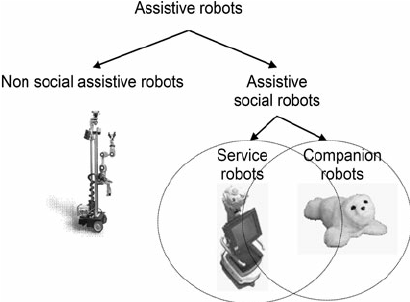
\includegraphics[scale=0.35]{gambar/kategori-sars.png}
  \caption{Pengategorian \emph{assistive robots} (\citet{cit:heerink2010}).}
  \label{fig:kategorisars}
\end{figure}

\emph{Socially assistive robots} (SARs) merupakan adaptasi dari \emph{assistive technology} yang meliputi keseluruhan sistem robotika yang mampu memberikan bantuan kepada pengguna dalam bentuk interaksi sosial \citep{cit:seifer2005}. \citet{cit:heerink2010} mengategorikan riset terhadap SARs menjadi dua kategori berbeda seperti pada Gambar \ref{fig:kategorisars}.
Kategori pertama mencakup \emph{service robots} yang menawarkan bantuan fisik dan kognitif dan melakukan tugas sebagai pelayan, sedangkan kategori kedua mencakup \emph{companion robot} yang merupakan robot berjenis pendamping sebagai sahabat dan media untuk terapi.

Lebih lanjut Rich dan Sidner \citep{cit:rich2009}, menjelaskan SARs mampu memberikan bantuan kepada pengguna dalam berbagai tingkatan seperti:
(a) mendukung kemampuan fungsional dan kognitif pengguna;
(b) menawarkan pengguna kesempatan untuk meningkatkan partisipasi sosial dan kesehatan psikologis;
(c) menyediakan pemantauan jarak jauh dan berkelanjutan atas status kesehatan pengguna;
dan (d) membina pengguna untuk memfasilitasi promosi perilaku sehat dan pencapaian tujuan yang berhubungan dengan kesehatan.
